\documentclass[preprint,aos]{imsart}
\usepackage{graphicx}
\usepackage{caption}
\usepackage{subcaption}
\usepackage{layouts} % \printinunitsof
\usepackage{booktabs}

\begin{document}

The most common file I used is \verb|\documentclass[preprint,aos]{imsart}|
and the \verb|\linewidth| is \printinunitsof{in}\prntlen{\linewidth},
\printinunitsof{cm}\prntlen{\linewidth}, \printinunitsof{pt}\prntlen{\linewidth},
\printinunitsof{bp}\prntlen{\linewidth}.

To be consistent about the unit used in different plotting, \emph{inch} 
is used as \verb|matplotlib| only use inches (integer). 
Another thing to note that 1 in is 72.27 pt while other is 72 pt.

The exact code to reproduce the plots in R and TikZ are in the same folder.
However, the TikZ did not output a pdf file at 2.8x2.1in despite explicit specification.
No solution is found so I will stick to R for the time being.

Between subfigure, a small spacing is added.

\begin{table}[ht]
\centering
\caption{Suggested width and height in cm for 4:3 aspect ratio}
\begin{tabular}{lcc}
\toprule
            & width & height \\
\midrule
Single plot & 12.8  & 9.6    \\
Two plots   & 6.4   & 4.8    \\
\bottomrule
\end{tabular}
\end{table}

\begin{figure}[htb]
    \centering
    \begin{subfigure}[t]{2.8in}
        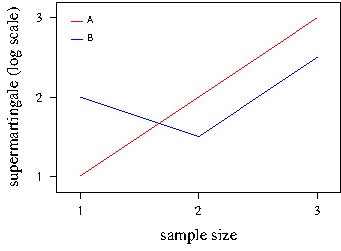
\includegraphics{scatterplot-tikz.pdf}
        \caption{TikZ}
    \end{subfigure}\hfill
    \begin{subfigure}[t]{2.8in}
        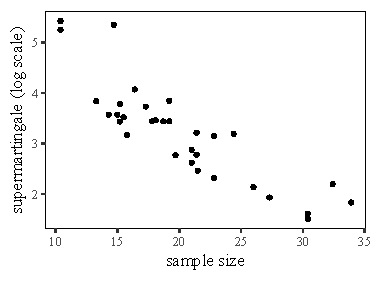
\includegraphics[width=2.8in]{scatterplot-R.pdf}
        \caption{R}
    \end{subfigure}

    \caption{TikZ vs R plots, exact physical size, no scaling.}
\end{figure}

\begin{figure}[htb]
    \centering
    \begin{subfigure}[t]{2.8in}
        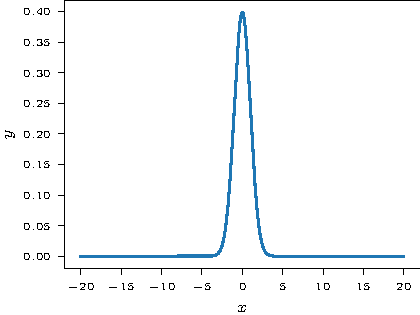
\includegraphics{scatterplot-python.pdf}
        \caption{Python}
    \end{subfigure}\hfill
    \begin{subfigure}[t]{2.8in}
        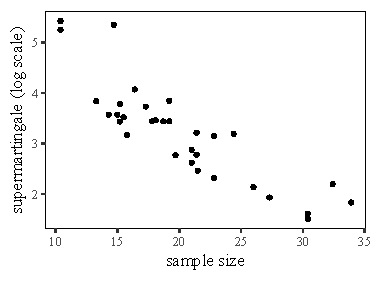
\includegraphics{scatterplot-R.pdf}
        \caption{R}
    \end{subfigure}

    \caption{Python vs R plots, exact physical size, no scaling.}
\end{figure}

The takeaway is that one should be consistent and it is extremely 
difficult to achieve such with different plotting languages.
This is on itself a \emph{strong} argument to plot everything 
in on project in R or TikZ or Python.

\end{document}